\hypertarget{usecase-ajax}{%
\chapter{ユースケース: Ajax通信}\label{usecase-ajax}}

ここではウェブブラウザ上でAjax通信をするユースケースとして、GitHubのユーザーIDからプロフィール情報を取得するアプリケーションを作成します。

作成するアプリケーションは次の要件を満たすものとします。

\begin{itemize}
\item
  GitHubのユーザーIDをテキストボックスに入力できる
\item
  入力されたユーザーIDを元にGitHubからユーザー情報を取得する
\item
  取得したユーザー情報をアプリケーション上で表示する
\end{itemize}

\hypertarget{entrypoint}{%
\section{エントリーポイント}\label{entrypoint}}

エントリーポイントとは、アプリケーションの中で一番最初に呼び出される部分のことです。
アプリケーションを作成するにあたり、まずはエントリーポイントを用意しなければなりません。

Webアプリケーションにおいては、常にHTMLドキュメントがエントリーポイントとなります。
ウェブブラウザによりHTMLドキュメントが読み込まれたあとに、HTMLドキュメント中で読み込まれたJavaScriptが実行されます。

\hypertarget{create-project-directory}{%
\subsection{プロジェクトディレクトリを作成}\label{create-project-directory}}

今回作成するアプリにはHTMLやJavaScriptなど複数のファイルが必要となります。
そのため、まずそれらのファイルを置くためのディレクトリを作成します。

ここでは \texttt{ajaxapp}
という名前で新しいディレクトリを作成します。ここからは作成した\texttt{ajaxapp}ディレクトリ以下で作業していきます。

またこのプロジェクトで作成するファイルは、必ず文字コード(エンコーディング)を\textbf{UTF-8}、改行コードを\textbf{LF}にしてファイルを保存します。

\hypertarget{preparing-html}{%
\subsection{HTMLファイルの用意}\label{preparing-html}}

エントリーポイントとして、まずは最低限の要素だけを配置したHTMLファイルを\texttt{index.html}というファイル名で作成しましょう。
\texttt{body}要素の一番下で読み込んでいる\texttt{index.js}が、今回のアプリケーションの処理を記述するJavaScriptファイルです。

\begin{listtitle}
index.html
\end{listtitle}
\begin{lstlisting}
<html lang="ja">
  <head>
    <meta charset="utf-8" />
    <title>Ajax Example</title>
  </head>
  <body>
    <h2>GitHub User Info</h2>
    <script src="index.js"></script>
  </body>
</html>
\end{lstlisting}
\listend

次に同じディレクトリに\texttt{index.js}というファイルを作成します。
\texttt{index.js}にはスクリプトが正しく読み込まれたことを確認できるよう、コンソールにログを出力する処理だけを書いておきます。

\begin{listtitle}
index.js
\end{listtitle}
\begin{lstlisting}
console.log("index.js: loaded");
\end{lstlisting}
\listend

ここでの\texttt{ajaxapp}ディレクトリのファイル配置は次のようになっていれば問題ありません。

\begin{lstlisting}
ajaxapp
├── index.html
└── index.js
\end{lstlisting}

次はこの\texttt{index.html}をブラウザで表示して、コンソールにログが出力されることを確認していきます。

\hypertarget{local-server}{%
\subsection{ローカルサーバーでHTMLを確認する}\label{local-server}}

ウェブブラウザで\texttt{index.html}を開く前に、開発用のローカルサーバーを準備します。
ローカルサーバーを立ち上げずに直接HTMLファイルを開くこともできますが、その場合は\texttt{file:///}からはじまるURLになります。
\texttt{file}スキーマでは\href{https://developer.mozilla.org/ja/docs/Web/Security/Same-origin_policy}{Same
Origin
Policy}のセキュリティ制限により、多くの場面でアプリケーションは正しく動作しません。
本章はローカルサーバーを立ち上げた上で、\texttt{http}スキーマのURLでアクセスすることを前提としています。

コマンドラインで\texttt{ajaxapp}ディレクトリへ移動し、次のコマンドでローカルサーバーを起動します。
次のコマンドでは、この書籍用に作成された\texttt{@js-primer/local-server}というローカルサーバーモジュールをダウンロードと同時に実行します。
まだ\texttt{npx}コマンドの用意ができていなければ、先に\href{../../setup-local-env/README.md}{アプリケーション開発の準備}を参照してください。

\begin{lstlisting}
$ npx @js-primer/local-server
\end{lstlisting}

起動したローカルサーバーのURL(\texttt{http://localhost:3000})へブラウザでアクセスすると、\texttt{"index.js: loaded"}とコンソールにログが出力されます。
Console
APIで出力したログを確認するには、ウェブブラウザの開発者ツールを開く必要があります。
ほとんどのブラウザで開発者ツールが同梱されていますが、本章ではFirefoxを使って確認します。
Firefoxの開発者ツールは次のいずれかの方法で開きます。

\begin{itemize}
\item
  Firefox メニュー(メニューバーがある場合や macOS
  では、ツールメニュー)の Web 開発サブメニューで ``Web コンソール''
  を選択する
\item
  キーボードショートカット Ctrl+Shift+K(macOS では
  Command+Option+K)を押下する
\end{itemize}

詳細は``\href{https://developer.mozilla.org/ja/docs/Tools/Web_Console/Opening_the_Web_Console}{Webコンソールを開く}''を参照してください。

\begin{figure}
\centering
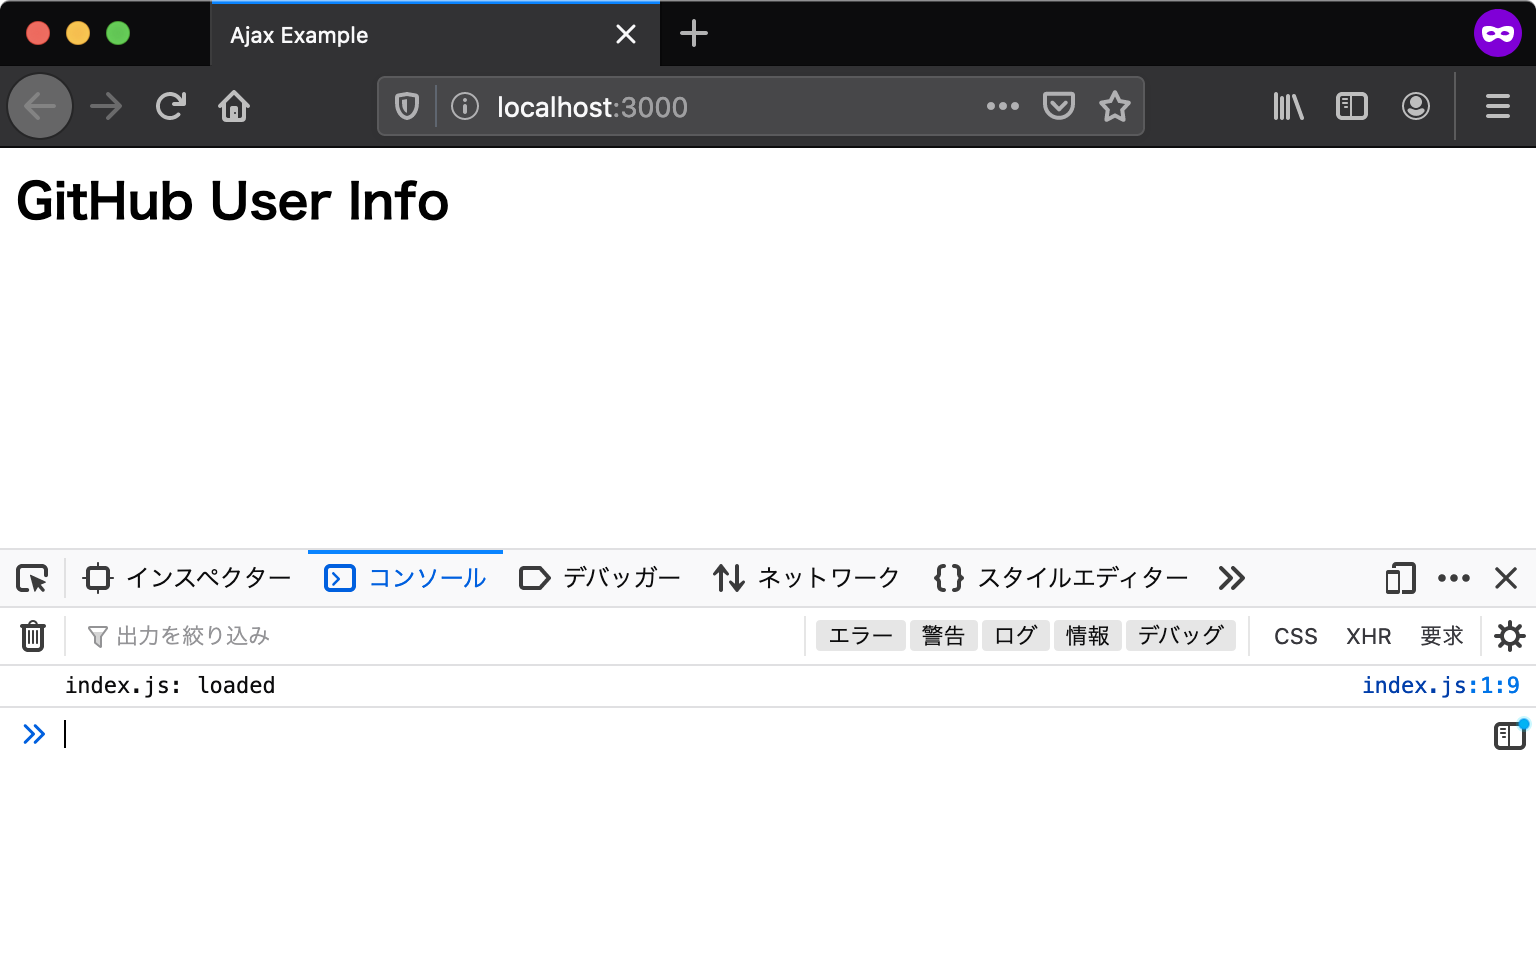
\includegraphics[width=120mm]{fig/fig-1.png}
\caption{ログが表示されているWebコンソール}
\end{figure}

\hypertarget{web-browsers-and-dom}{%
\subsection{ウェブブラウザとDOM}\label{web-browsers-and-dom}}

HTMLドキュメントをブラウザで読み込むとき、\href{https://developer.mozilla.org/ja/docs/Web/API/Document_Object_Model/Introduction}{DOM}と呼ばれるプログラミング用のデータ表現が生成されます。
\textbf{DOM(Document Object Model)}
とは、HTMLドキュメントのコンテンツと構造をJavaScriptから操作できるオブジェクトです。
DOMではHTMLドキュメントのタグの入れ子関係を木構造で表現するため、DOMが表現するHTMLタグの木構造を
\textbf{DOMツリー} と呼びます。

たとえば、DOMにはHTMLドキュメントそのものを表現する
\texttt{document} グローバルオブジェクトがあります。
\texttt{document}
グローバルオブジェクトには、指定したHTML要素を取得したり、新しくHTML要素を作成するメソッドが実装されています。
\texttt{document}
グローバルオブジェクトを使うことで、先ほどの\texttt{index.html}
に書かれたHTMLをJavaScriptから操作できます。

\begin{lstlisting}
// CSSセレクタを使ってDOMツリー中のh2要素を取得する
const heading = document.querySelector("h2");
// h2要素に含まれるテキストコンテンツを取得する
const headingText = heading.textContent;

// button要素を作成する
const button = document.createElement("button");
button.textContent = "Push Me";
// body要素の子要素としてbuttonを挿入する
document.body.appendChild(button);
\end{lstlisting}

JavaScriptとDOMはWebアプリケーション開発において切っても切り離せない関係です。
動的なWebアプリケーションを作るためには、JavaScriptによるDOMの操作が不可欠です。
今回のユースケースでもGitHubのAPIから取得したデータを元に、動的にDOMツリーを操作して画面の表示を更新します。

しかし、DOMは言語機能(ECMAScript)ではなくブラウザが実装しているAPIです。
そのため、DOMを持たないNode.jsなどの実行環境では使えず、\texttt{document}のようなグローバルオブジェクトも存在しないことには注意が必要です。

\hypertarget{section-checklist}{%
\subsection{このセクションのチェックリスト}\label{section-checklist}}

このセクションでは、エントリーポイントとなるHTMLを作成し、JavaScriptモジュールのエントリーポイントとなるJavaScriptファイルを読み込むところまでを実装しました。

\begin{itemize}
\item
  \texttt{ajaxapp}という名前のプロジェクトディレクトリを作成した
\item
  エントリーポイントとなる\texttt{index.html}を作成した
\item
  JavaScriptのエントリーポイントとなる\texttt{index.js}を作成し\texttt{index.html}から読み込んだ
\item
  ローカルサーバーを使ってブラウザで\texttt{index.html}を表示した
\item
  \texttt{index.js}からコンソールに出力されたログを確認した
\item
  JavaScriptからHTMLドキュメントを操作するDOMについて学んだ
\end{itemize}

\hypertarget{http-communication}{%
\section{HTTP通信}\label{http-communication}}

ローカルサーバーでアプリケーションが実行できるようになったので、次はGitHubのAPIを呼び出す処理を実装していきます。
GitHubのAPIを呼び出すためにはHTTP通信をする必要があります。
ウェブブラウザ上でJavaScriptからHTTP通信するために、\href{https://developer.mozilla.org/ja/docs/Web/API/Fetch_API}{Fetch
API}という機能を使います。

\hypertarget{fetch-api}{%
\subsection{Fetch API}\label{fetch-api}}

\textbf{Fetch API}はHTTP通信を行ってリソースを取得するためのAPIです。
Fetch
APIを使うことで、ページ全体を再読み込みすることなく指定したURLからデータを取得できます。
Fetch
APIは同じくHTTP通信を扱う\href{https://developer.mozilla.org/ja/docs/Web/API/XMLHttpRequest}{XMLHttpRequest}と似たAPIですが、より強力で柔軟な操作が可能です。

リクエストを送信するためには、\texttt{fetch}メソッドを利用します。
\texttt{fetch}メソッドにURLを与えることで、HTTPリクエストが作成され、サーバーとのHTTP通信を開始します。

GitHubにはユーザー情報を取得するAPIとして、\texttt{https://api.github.com/users/GitHubユーザーID}というURLが用意されています。
GitHubのユーザーIDには、英数字と\texttt{-}(ハイフン)以外は利用できないため、ユーザーIDは\texttt{encodeURIComponent}関数を使ってエスケープしたものを結合します。\texttt{encodeURIComponent}は\texttt{/}や\texttt{\%}などURLとして特殊な意味を持つ文字列をただの文字列として扱えるようにエスケープする関数です。

次のコードでは、指定したGitHubユーザーIDの情報を取得するURLに対して\texttt{fetch}メソッドで、GETのHTTPリクエストを行っています。

\begin{lstlisting}
const userId = "任意のGitHubユーザーID";
fetch(`https://api.github.com/users/${encodeURIComponent(userId)}`);
\end{lstlisting}

\hypertarget{receive-response}{%
\subsection{レスポンスの受け取り}\label{receive-response}}

GitHubのAPIに対してHTTPリクエストを送信しましたが、まだレスポンスを受け取る処理を書いていません。
次はサーバーから返却されたレスポンスのログをコンソールに出力する処理を実装します。

\texttt{fetch}メソッドは\texttt{Promise}を返します。この\texttt{Promise}インスタンスはリクエストのレスポンスを表す\texttt{Response}オブジェクトでresolveされます。
送信したリクエストにレスポンスが返却されると、\texttt{then}コールバックが呼び出されます。

次のように、\texttt{Response}オブジェクトの\texttt{status}プロパティからは、HTTPレスポンスのステータスコードが取得できます。
また、\texttt{Response}オブジェクトの\texttt{json}メソッドも\texttt{Promise}を返します。これは、HTTPレスポンスボディをJSONとしてパースしたオブジェクトでresolveされます。
ここでは、書籍用に用意した\texttt{js-primer-example}というGitHubアカウントのユーザー情報を取得しています。

\begin{lstlisting}
const userId = "js-primer-example";
fetch(`https://api.github.com/users/${encodeURIComponent(userId)}`)
    .then(response => {
        console.log(response.status); // => 200
        return response.json().then(userInfo => {
            // JSONパースされたオブジェクトが渡される
            console.log(userInfo); // => {...}
        });
    });
\end{lstlisting}

\hypertarget{error-handling}{%
\subsection{エラーハンドリング}\label{error-handling}}

HTTP通信にはエラーがつきものです。 そのためFetch
APIを使った通信においても、エラーをハンドリングする必要があります。
たとえば、サーバーとの通信に際してネットワークエラーが発生した場合は、ネットワークエラーを表す\texttt{NetworkError}オブジェクトでrejectされた\texttt{Promise}が返されます。
すなわち、\texttt{then}メソッドの第二引数か\texttt{catch}メソッドのコールバック関数が呼び出されます。

\begin{lstlisting}
const userId = "js-primer-example";
fetch(`https://api.github.com/users/${encodeURIComponent(userId)}`)
    .then(response => {
        console.log(response.status);
        return response.json().then(userInfo => {
            console.log(userInfo);
        });
    }).catch(error => {
        console.error(error);
    });
\end{lstlisting}

一方で、リクエストが成功したかどうかは\texttt{Response}オブジェクトの\texttt{ok}プロパティで認識できます。
\texttt{ok}プロパティは、HTTPステータスコードが200番台であれば\texttt{true}を返し、それ以外の400や500番台などなら\texttt{false}を返します。
次のように、\texttt{ok}プロパティが\texttt{false}となるエラーレスポンスをハンドリングできます。

\begin{lstlisting}
const userId = "js-primer-example";
fetch(`https://api.github.com/users/${encodeURIComponent(userId)}`)
    .then(response => {
        console.log(response.status); 
        // エラーレスポンスが返されたことを検知する
        if (!response.ok) {
            console.error("エラーレスポンス", response);
        } else {
            return response.json().then(userInfo => {
                console.log(userInfo);
            });
        }
    }).catch(error => {
        console.error(error);
    });
\end{lstlisting}

ここまでの内容をまとめ、GitHubからユーザー情報を取得する関数を\texttt{fetchUserInfo}という名前で定義します。

\begin{lstlisting}
function fetchUserInfo(userId) {
    fetch(`https://api.github.com/users/${encodeURIComponent(userId)}`)
        .then(response => {
            console.log(response.status);
            // エラーレスポンスが返されたことを検知する
            if (!response.ok) {
                console.error("エラーレスポンス", response);
            } else {
                return response.json().then(userInfo => {
                    console.log(userInfo);
                });
            }
        }).catch(error => {
            console.error(error);
        });
}
\end{lstlisting}

index.jsでは関数を定義しているだけで、呼び出しは行っていません。

ページを読み込むたびにGitHubのAPIを呼び出すと、呼び出し回数の制限を超えるおそれがあります。
呼び出し回数の制限を超えると、APIからのレスポンスがステータスコード403のエラーになってしまいます。

そのため、HTMLドキュメント側に手動で\texttt{fetchUserInfo}関数を呼び出すためのボタンを追加します。
ボタンのclickイベントで\texttt{fetchUserInfo}関数を呼び出し、取得したいユーザーIDを引数として与えています。
例として\texttt{js-primer-example}という書籍用に用意したGitHubアカウントを指定しています。

\begin{lstlisting}
<html lang="ja">
  <head>
    <meta charset="utf-8" />
    <title>Ajax Example</title>
  </head>
  <body>
    <h2>GitHub User Info</h2>

    <button onclick="fetchUserInfo('js-primer-example');">Get user info</button>
    <script src="index.js"></script>
  </body>
</html>
\end{lstlisting}

準備ができたら、ローカルサーバーを立ち上げてindex.htmlにアクセスしましょう。
ボタンを押すとHTTP通信が行われ、コンソールにステータスコードとレスポンスのログが出力されます。

\begin{figure}
\centering
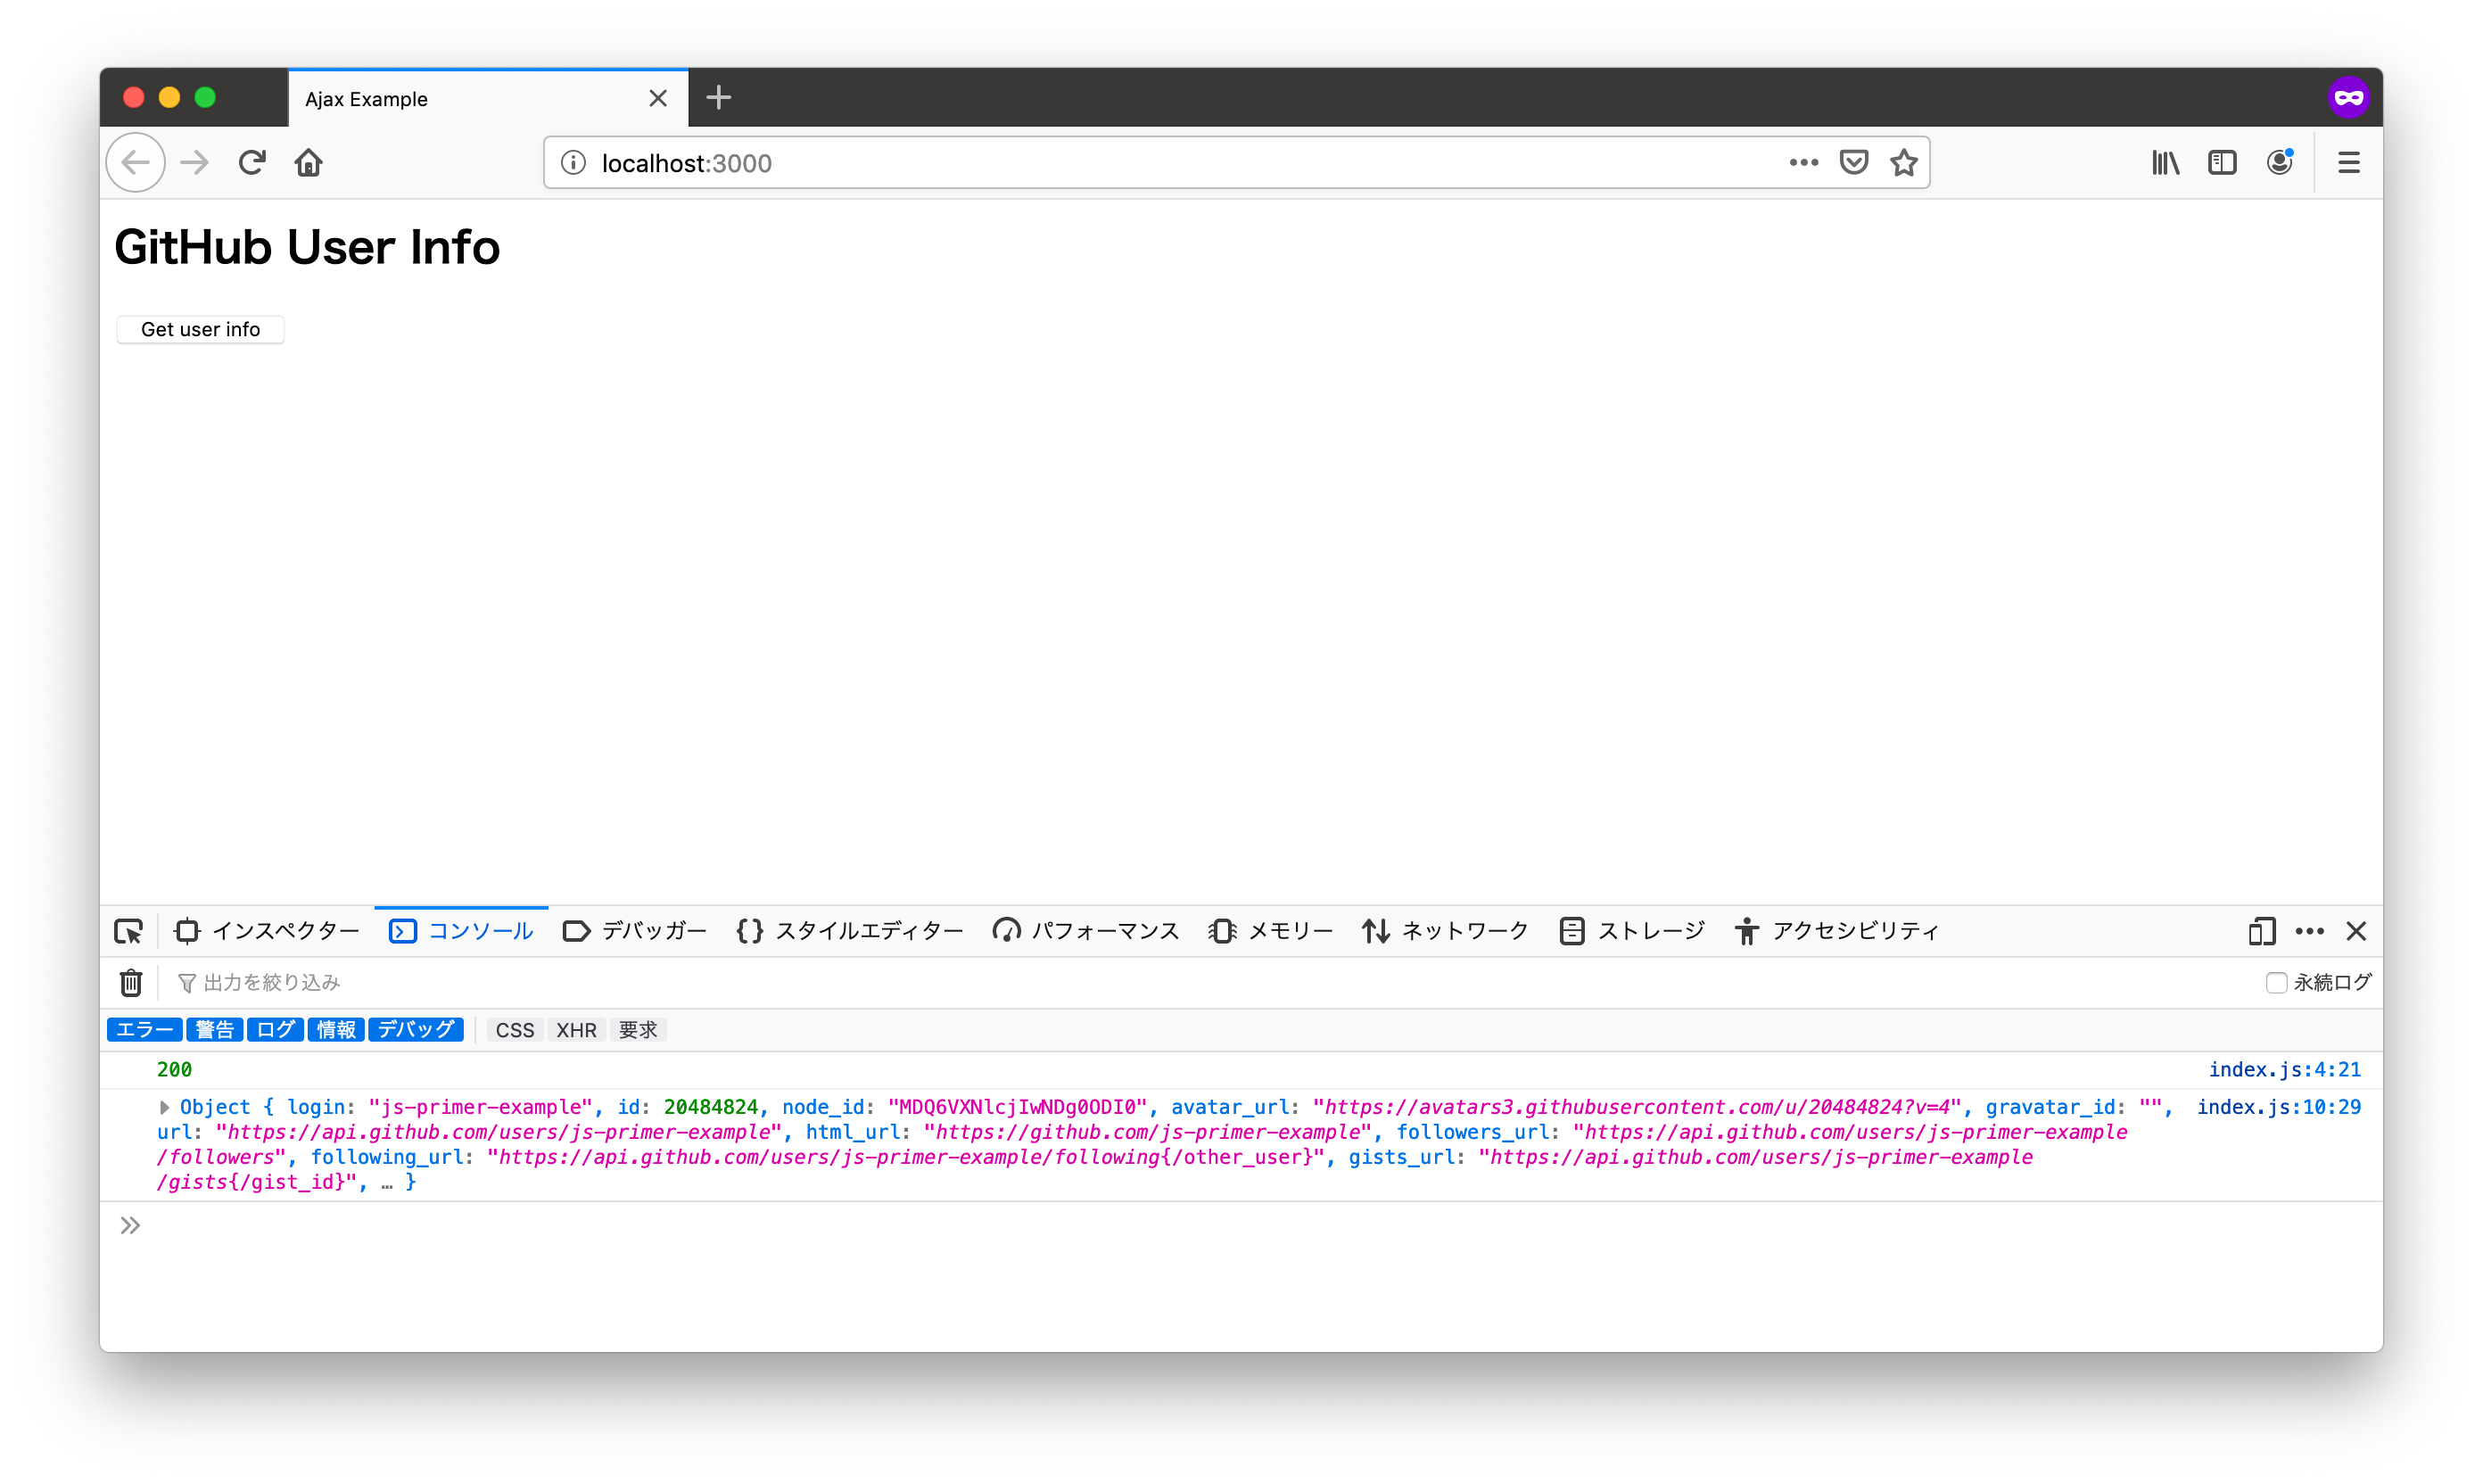
\includegraphics[width=120mm]{fig/fig-2.png}
\caption{Fetchで取得したデータの表示}
\end{figure}

また、開発者ツールのネットワークパネルを開くと、GitHubのサーバーに対してHTTP通信が行われていることを確認できます。

\begin{figure}
\centering
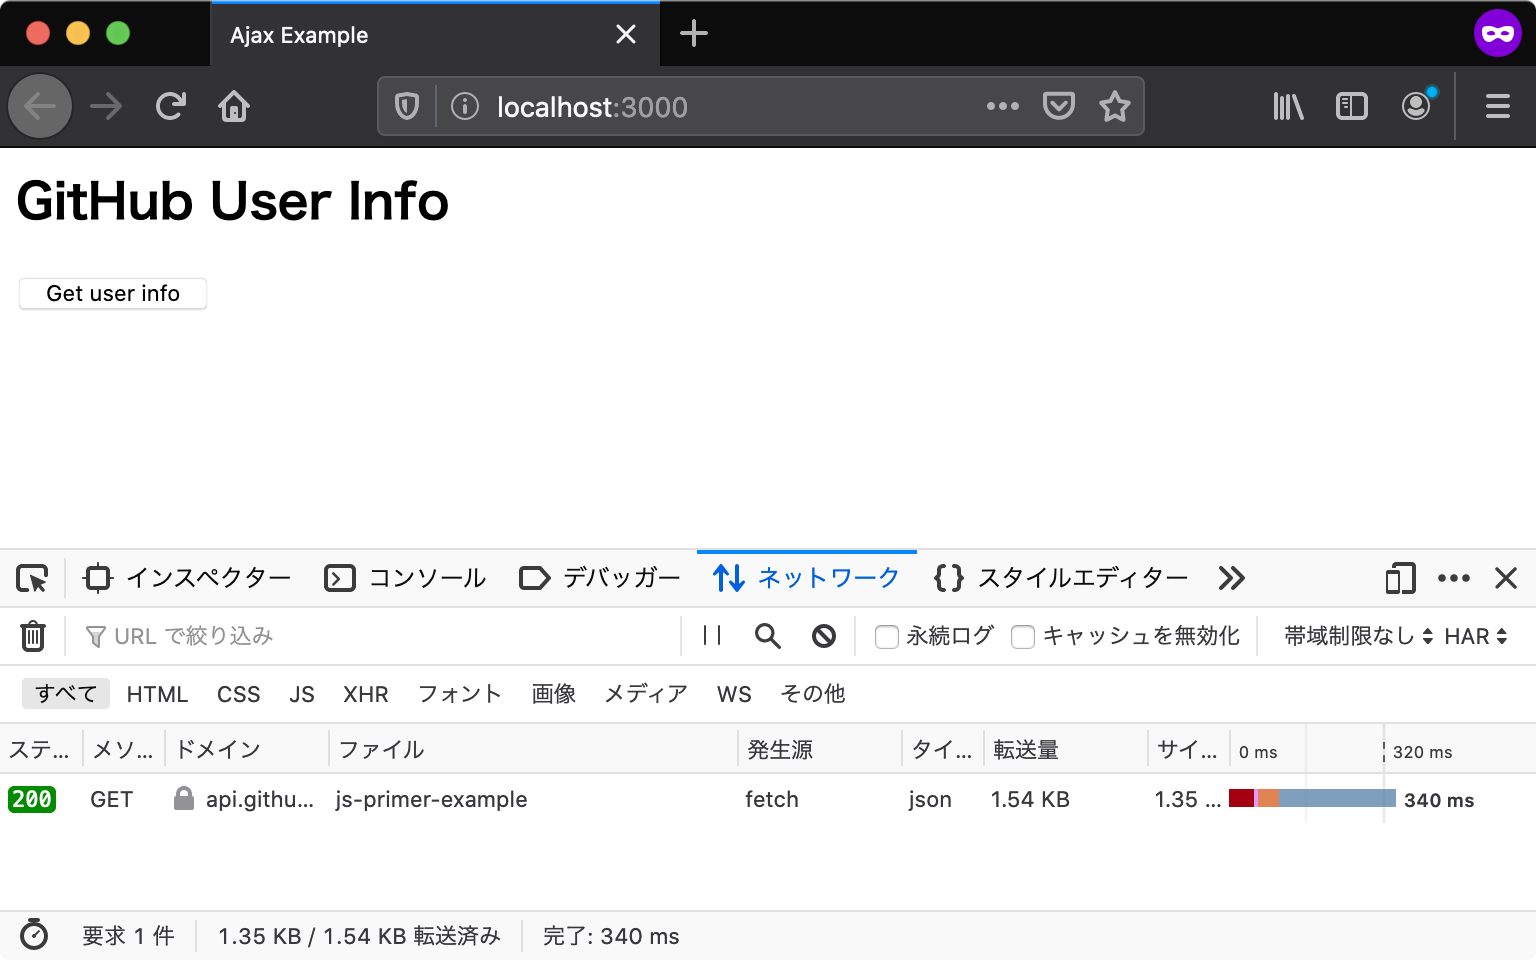
\includegraphics[width=120mm]{fig/fig-3.png}
\caption{開発者ツールでHTTP通信の記録を確認する}
\end{figure}

\begin{tcolorbox}[title=XMLHttpRequest]\label{xhr}

\href{https://developer.mozilla.org/ja/docs/Web/API/XMLHttpRequest}{XMLHttpRequest}(\textbf{XHR})はFetch
APIと同じくHTTP通信を行うためのAPIです。 Fetch
APIが標準化される以前は、ブラウザとサーバーの間で通信を行うにはXHRを使うのが一般的でした。
このセクションで扱ったFetch
APIによる\texttt{fetchUserInfo}関数は、XHRを使うと次のように書けます。

\begin{lstlisting}
function fetchUserInfo(userId) {
    // リクエストを作成する
    const request = new XMLHttpRequest();
    request.open("GET", `https://api.github.com/users/${encodeURIComponent(userId)}`);
    request.addEventListener("load", () => {
        // リクエストが成功したかを判定する
        // Fetch APIのresponse.okと同等の意味
        if (request.status >= 200 && request.status < 300) {
            // レスポンス文字列をJSONオブジェクトにパースする
            const userInfo = JSON.parse(request.responseText);
            console.log(userInfo);
        } else {
            console.error("エラーレスポンス", request.statusText);
        }
    });
    request.addEventListener("error", () => {
        console.error("ネットワークエラー");
    });
    // リクエストを送信する
    request.send();
}
\end{lstlisting}

Fetch
APIはXHRを置き換えるために作られたもので、多くのユースケースではXHRを使う必要はなくなっています。
ただし、古いブラウザではFetch
APIが実装されていないため、ブラウザの互換性を保つためにXHRを使う場面もまだあります。
XHRの詳しい使い方については、\href{https://developer.mozilla.org/ja/docs/Web/API/XMLHttpRequest/Using_XMLHttpRequest}{XHRの利用についてのドキュメント}を参照してください。
\end{tcolorbox}

\hypertarget{section-checklist}{%
\subsection{このセクションのチェックリスト}\label{section-checklist}}

\begin{itemize}
\item
  \href{https://developer.mozilla.org/ja/docs/Web/API/Fetch_API}{Fetch
  API}を使ってHTTPリクエストを送った
\item
  GitHubのAPIから取得したユーザー情報のJSONオブジェクトをコンソールに出力した
\item
  Fetch APIの呼び出しに対するエラーハンドリングを行った
\item
  \texttt{fetchUserInfo}関数を宣言し、ボタンのクリックイベントで呼び出した
\end{itemize}

\hypertarget{display-data}{%
\section{データを表示する}\label{display-data}}

前のセクションでは、Fetch
APIを使ってGitHubのAPIからユーザー情報を取得しました。
このセクションでは取得したデータをHTMLに整形して、アプリケーションにユーザー情報を表示してみましょう。

\hypertarget{markup-html}{%
\subsection{HTMLを組み立てる}\label{markup-html}}

HTML文字列の生成にはテンプレートリテラルを使います。
テンプレートリテラルは文字列中の改行が可能なため、HTMLのインデントを表現できて見通しが良くなります。
また、変数の埋め込みも簡単なため、HTMLのテンプレートに対して動的なデータをあてはめるのに適しています。

次のコードではGitHubのユーザー情報から組み立てるHTMLのテンプレートを宣言しています。

\begin{lstlisting}
const view = `
<h4>${userInfo.name} (@${userInfo.login})</h4>
<img src="${userInfo.avatar_url}" alt="${userInfo.login}" height="100">
<dl>
    <dt>Location</dt>
    <dd>${userInfo.location}</dd>
    <dt>Repositories</dt>
    <dd>${userInfo.public_repos}</dd>
</dl>
`;
\end{lstlisting}

このテンプレートに\texttt{userInfo}オブジェクトの値をあてはめると、次のようなHTML文字列になります。

\begin{lstlisting}[language=HTML]
<h4>js-primer example (@js-primer-example)</h4>
<img src="https://github.com/js-primer-example.png" alt="js-primer-example" height="100">
<dl>
    <dt>Location</dt>
    <dd>Japan</dd>
    <dt>Repositories</dt>
    <dd>1</dd>
</dl>
\end{lstlisting}

\hypertarget{html-to-dom}{%
\subsection{HTML文字列をDOMに追加する}\label{html-to-dom}}

次に、生成したHTML文字列をDOMツリーに追加して表示します。
まずは動的にHTMLをセットするために、目印となる要素を\texttt{index.html}に追加します。
今回は\texttt{result}というidを持ったdiv要素(以降\texttt{div\#result}と表記します)を配置します。

\begin{listtitle}
index.html
\end{listtitle}
\begin{lstlisting}
<html lang="ja">
  <head>
    <meta charset="utf-8" />
    <title>Ajax Example</title>
  </head>
  <body>
    <h2>GitHub User Info</h2>

    <button onclick="fetchUserInfo('js-primer-example');">Get user info</button>
    <!-- 整形したHTMLの挿入先 -->
    <div id="result"></div>

    <script src="index.js"></script>
  </body>
</html>
\end{lstlisting}
\listend

ここから、\texttt{div\#result}要素の子要素としてHTML文字列を挿入することになります。
\href{https://developer.mozilla.org/ja/docs/Web/API/Document/getElementById}{document.getElementById}メソッドを使い、id属性が設定された要素にアクセスします。
\texttt{div\#result}要素が取得できたら、先ほど生成したHTML文字列を\texttt{innerHTML}プロパティにセットします。

\begin{lstlisting}
const result = document.getElementById("result");
result.innerHTML = view;
\end{lstlisting}

JavaScriptによってHTML要素をDOMに追加する方法には、大きく分けて2つあります。
1つは、今回のようにHTML文字列を\href{https://developer.mozilla.org/ja/docs/Web/API/Element/innerHTML}{Element\#innerHTML}プロパティにセットする方法です。
もう1つは、文字列ではなく\href{https://developer.mozilla.org/ja/docs/Web/API/Element}{Element}オブジェクトを生成して\href{https://developer.mozilla.org/ja/docs/Web/API/Node/appendChild}{手続き的にツリー構造を構築する}方法です。
後者はセキュリティ的に安全ですが、コードは少し冗長になります。
今回は\texttt{Element\#innerHTML}プロパティを使いつつ、セキュリティのためのエスケープ処理を行います。

\hypertarget{escape-html}{%
\subsection{HTML文字列をエスケープする}\label{escape-html}}

\texttt{Element\#innerHTML}に文字列をセットすると、その文字列はHTMLとして解釈されます。
たとえばGitHubのユーザー名に\texttt{<}記号や\texttt{>}記号が含まれていると、意図しない構造のHTMLになる可能性があります。
これを回避するために、文字列をセットする前に、特定の記号を安全な表現に置換する必要があります。
この処理を一般にHTMLのエスケープと呼びます。

多くのViewライブラリは内部にエスケープ機構を持っていて、動的にHTMLを組み立てるときにはデフォルトでエスケープをしてくれます。
または、\href{https://github.com/teppeis/htmlspecialchars}{エスケープ用のライブラリ}を利用するケースも多いでしょう。
今回のように独自実装するのは特別なケースで、一般的にはライブラリが提供する機能を使うのがほとんどです。

次のように、特殊な記号に対するエスケープ処理を\texttt{escapeSpecialChars}関数として宣言します。

\begin{lstlisting}
function escapeSpecialChars(str) {
    return str
        .replace(/&/g, "&amp;")
        .replace(/</g, "&lt;")
        .replace(/>/g, "&gt;")
        .replace(/"/g, "&quot;")
        .replace(/'/g, "&#039;");
}
\end{lstlisting}

この\texttt{escapeSpecialChars}関数を、HTML文字列の中で\texttt{userInfo}から値を注入しているすべての箇所で行います。
ただし、テンプレートリテラル中で挿入している部分すべてに関数を適用するのは手間ですし、メンテナンス性もよくありません。
そこで、\href{https://developer.mozilla.org/ja/docs/Web/JavaScript/Reference/template_strings\#タグづけされたTemplate_literal}{テンプレートリテラルをタグづけ}することで、明示的にエスケープ用の関数を呼び出す必要がないようにします。
タグづけされたテンプレートリテラルは、テンプレートによる値の埋め込みを関数の呼び出しとして扱えます。

次の\texttt{escapeHTML}関数はテンプレートリテラルにタグづけするための\textbf{タグ関数}です。
タグ関数には、第一引数に文字列リテラルの配列、第二引数に埋め込まれる値の配列が与えられます。
\texttt{escapeHTML}関数では、文字列リテラルと値が元の順番どおりに並ぶように文字列を組み立てつつ、
値が文字列型であればエスケープするようにしています。

\begin{lstlisting}
function escapeHTML(strings, ...values) {
    return strings.reduce((result, str, i) => {
        const value = values[i - 1];
        if (typeof value === "string") {
            return result + escapeSpecialChars(value) + str;
        } else {
            return result + String(value) + str;
        }
    });  
}
\end{lstlisting}

\texttt{escapeHTML}関数はタグ関数なので、通常の\texttt{()}による呼び出しではなく、テンプレートリテラルに対してタグづけして使います。
テンプレートリテラルのバッククォート記号の前に関数を書くと、関数がタグづけされます。

\begin{lstlisting}
const view = escapeHTML`
<h4>${userInfo.name} (@${userInfo.login})</h4>
<img src="${userInfo.avatar_url}" alt="${userInfo.login}" height="100">
<dl>
    <dt>Location</dt>
    <dd>${userInfo.location}</dd>
    <dt>Repositories</dt>
    <dd>${userInfo.public_repos}</dd>
</dl>
`;

const result = document.getElementById("result");
result.innerHTML = view;
\end{lstlisting}

これでHTML文字列の生成とエスケープができました。
これらの処理を前のセクションで作成した
\texttt{fetchUserInfo} 関数の中で呼び出します。
ここまでで、index.jsとindex.htmlは次のようになっています。

\begin{listtitle}
index.js
\end{listtitle}
\begin{lstlisting}
function fetchUserInfo(userId) {
    fetch(`https://api.github.com/users/${encodeURIComponent(userId)}`)
        .then(response => {
            if (!response.ok) {
                console.error("エラーレスポンス", response);
            } else {
                return response.json().then(userInfo => {
                    // HTMLの組み立て
                    const view = escapeHTML`
                    <h4>${userInfo.name} (@${userInfo.login})</h4>
                    <img src="${userInfo.avatar_url}" alt="${userInfo.login}" height="100">
                    <dl>
                        <dt>Location</dt>
                        <dd>${userInfo.location}</dd>
                        <dt>Repositories</dt>
                        <dd>${userInfo.public_repos}</dd>
                    </dl>
                    `;
                    // HTMLの挿入
                    const result = document.getElementById("result");
                    result.innerHTML = view;
                });
            }
        }).catch(error => {
            console.error(error);
        });
}

function escapeSpecialChars(str) {
    return str
        .replace(/&/g, "&amp;")
        .replace(/</g, "&lt;")
        .replace(/>/g, "&gt;")
        .replace(/"/g, "&quot;")
        .replace(/'/g, "&#039;");
}

function escapeHTML(strings, ...values) {
    return strings.reduce((result, str, i) => {
        const value = values[i - 1];
        if (typeof value === "string") {
            return result + escapeSpecialChars(value) + str;
        } else {
            return result + String(value) + str;
        }
    });
}
\end{lstlisting}
\listend

\begin{listtitle}
index.html
\end{listtitle}
\begin{lstlisting}
<html lang="ja">
  <head>
    <meta charset="utf-8" />
    <title>Ajax Example</title>
  </head>
  <body>
    <h2>GitHub User Info</h2>

    <button onclick="fetchUserInfo('js-primer-example');">Get user info</button>
    <!-- 整形したHTMLの挿入先 -->
    <div id="result"></div>

    <script src="index.js"></script>
  </body>
</html>
\end{lstlisting}
\listend

アプリケーションを開いてボタンを押すと、次のようにユーザー情報が表示されます。

\begin{figure}
\centering
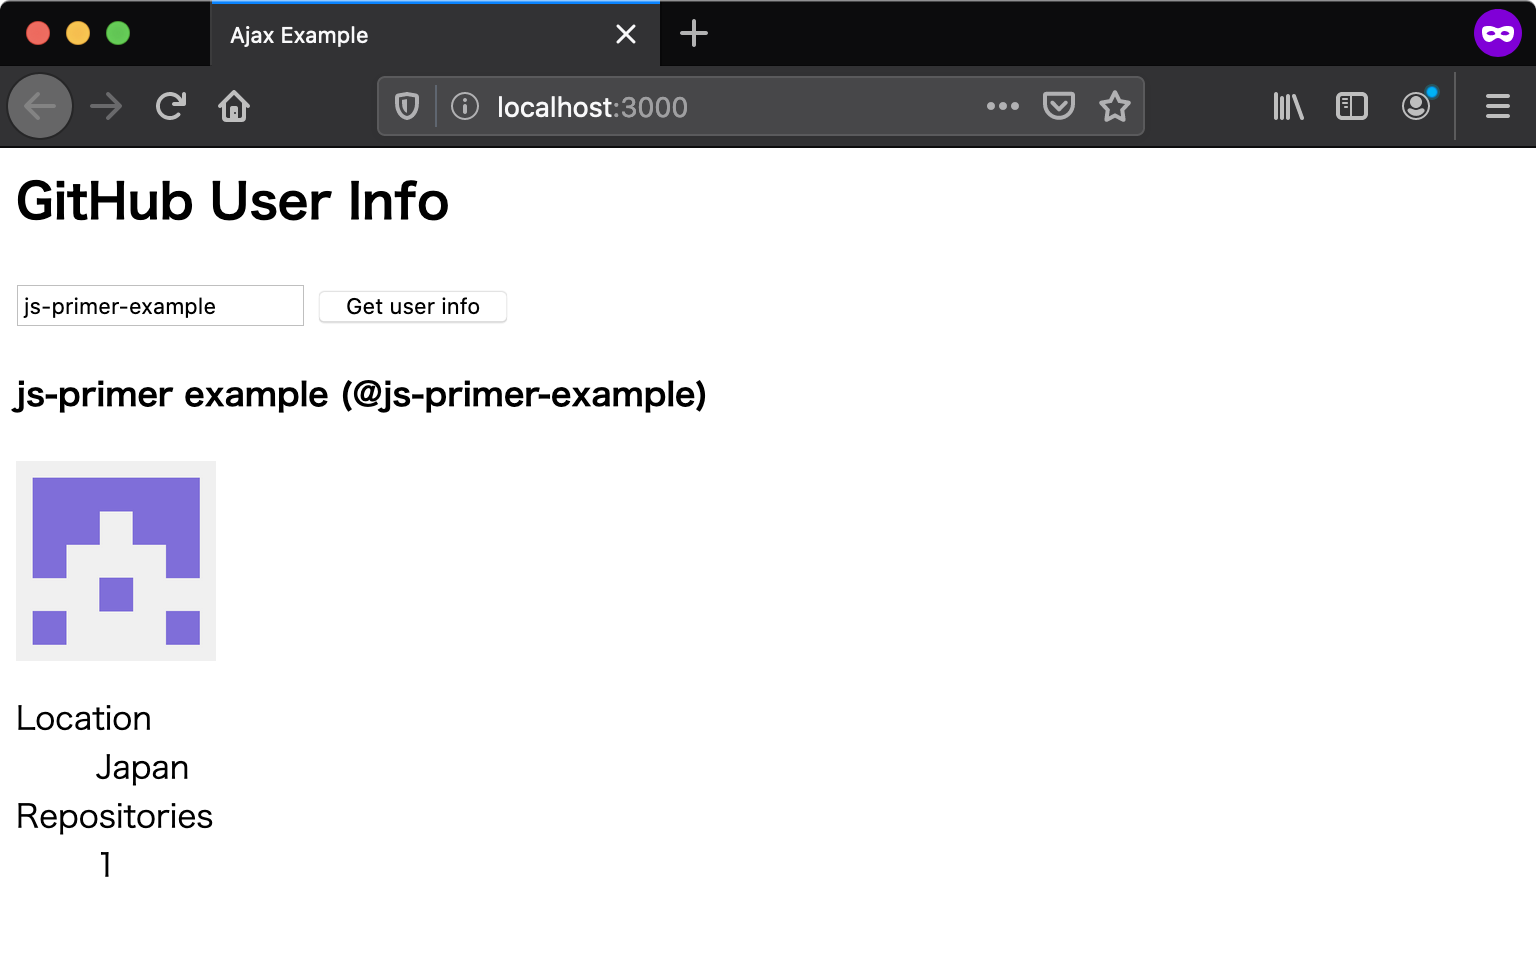
\includegraphics[width=100mm]{fig/fig-4.png}
\caption{ユーザー情報の表示}
\end{figure}

\hypertarget{section-checklist}{%
\subsection{このセクションのチェックリスト}\label{section-checklist}}

\begin{itemize}
\item
  \href{../../../basic/string/README.md\#create}{テンプレートリテラル}を使ってHTML文字列を組み立てた
\item
  \texttt{innerHTML}プロパティを使ってHTML文字列をDOMに追加した
\item
  {[}タグつきテンプレート関数{]}{[}{]}を使ってHTML文字列をエスケープした
\item
  \texttt{fetchUserInfo}関数を呼び出し、HTMLにユーザー情報が表示されることを確認した
\end{itemize}

\hypertarget{use-promise}{%
\section{Promiseを活用する}\label{use-promise}}

ここまでのセクションで、Fetch
APIを使ってAjax通信を行い、サーバーから取得したデータを表示できました。
最後に、Fetch
APIの戻り値でもある\textbf{Promise}を活用してソースコードを整理することで、エラーハンドリングをしっかり行います。

\hypertarget{split-function}{%
\subsection{関数の分割}\label{split-function}}

まずは、大きくなりすぎた\texttt{fetchUserInfo}関数を整理しましょう。
この関数では、Fetch
APIを使ったデータの取得・HTML文字列の組み立て・組み立てたHTMLの表示をしています。
そこで、HTML文字列を組み立てる\texttt{createView}関数とHTMLを表示する\texttt{displayView}関数を作り、処理を分割します。

また、後述するエラーハンドリングを行いやすくするため、アプリケーションにエントリーポイントを設けます。
\texttt{index.js}に新しく\texttt{main}関数を作り、\texttt{main}関数から\texttt{fetchUserInfo}関数を呼び出すようにします。

\begin{lstlisting}
function main() {
    fetchUserInfo("js-primer-example");
}

function fetchUserInfo(userId) {
    fetch(`https://api.github.com/users/${encodeURIComponent(userId)}`)
        .then(response => {
            if (!response.ok) {
                console.error("エラーレスポンス", response);
            } else {
                return response.json().then(userInfo => {
                    // HTMLの組み立て
                    const view = createView(userInfo);
                    // HTMLの挿入
                    displayView(view);
                });
            }
        }).catch(error => {
            console.error(error);
        });
}

function createView(userInfo) {
    return escapeHTML`
    <h4>${userInfo.name} (@${userInfo.login})</h4>
    <img src="${userInfo.avatar_url}" alt="${userInfo.login}" height="100">
    <dl>
        <dt>Location</dt>
        <dd>${userInfo.location}</dd>
        <dt>Repositories</dt>
        <dd>${userInfo.public_repos}</dd>
    </dl>
    `;
}

function displayView(view) {
    const result = document.getElementById("result");
    result.innerHTML = view;
}
\end{lstlisting}

ボタンのclickイベントで呼び出す関数もこれまでの\texttt{fetchUserInfo}関数から\texttt{main}関数に変更します。

\begin{listtitle}
index.html
\end{listtitle}
\begin{lstlisting}
<html lang="ja">
  <head>
    <meta charset="utf-8" />
    <title>Ajax Example</title>
  </head>
  <body>
    <h2>GitHub User Info</h2>

    <input id="userId" type="text" value="js-primer-example" />
    <button onclick="main();">Get user info</button>

    <div id="result"></div>

    <script src="index.js"></script>
  </body>
</html>
\end{lstlisting}
\listend

\hypertarget{error-handling}{%
\subsection{Promiseのエラーハンドリング}\label{error-handling}}

次に\texttt{fetchUserInfo}関数を変更し、Fetch
APIの戻り値でもあるPromiseオブジェクトを\texttt{return}します。
この変更によって、\texttt{fetchUserInfo}関数を呼び出す\texttt{main}関数のほうで非同期処理の結果を扱えるようになります。
Promiseチェーンの中で投げられたエラーは、\texttt{Promise\#catch}メソッドを使って一箇所で受け取れます。

次のコードでは、\texttt{fetchUserInfo}関数から返されたPromiseオブジェクトを、\texttt{main}関数でエラーハンドリングしてログを出力します。
\texttt{fetchUserInfo}関数の\texttt{catch}メソッドでハンドリングしていたエラーは、\texttt{main}関数の\texttt{catch}メソッドでハンドリングされます。
一方、\texttt{Response\#ok}で判定していた400や500などのエラーレスポンスがそのままでは\texttt{main}関数でハンドリングできません。
そこで、\texttt{Promise.reject}メソッドを使ってRejectedなPromiseを返し、Promiseチェーンをエラーの状態にします。
Promiseチェーンがエラーとなるため、\texttt{main}関数の\texttt{catch}でハンドリングできます。

\begin{lstlisting}
function main() {
    fetchUserInfo("js-primer-example")
        .catch((error) => {
            // Promiseチェーンの中で発生したエラーを受け取る
            console.error(`エラーが発生しました (${error})`);
        });
}

function fetchUserInfo(userId) {
    // fetchの戻り値のPromiseをreturnする
    return fetch(`https://api.github.com/users/${encodeURIComponent(userId)}`)
        .then(response => {
            if (!response.ok) {
                // エラーレスポンスからRejectedなPromiseを作成して返す
                return Promise.reject(new Error(`${response.status}: ${response.statusText}`));
            } else {
                return response.json().then(userInfo => {
                    // HTMLの組み立て
                    const view = createView(userInfo);
                    // HTMLの挿入
                    displayView(view);
                });
            }
        });
}
\end{lstlisting}

\hypertarget{refactor-promise-chain}{%
\subsubsection{Promiseチェーンのリファクタリング}\label{refactor-promise-chain}}

現在の\texttt{fetchUserInfo}関数はデータの取得に加えて、HTMLの組み立て(\texttt{createView})と表示(\texttt{displayView})も行っています。
\texttt{fetchUserInfo}関数に処理が集中して見通しが悪いため、\texttt{fetchUserInfo}関数はデータの取得だけを行うように変更します。
併せて\texttt{main}関数で、データの取得(\texttt{fetchUserInfo})、HTMLの組み立て(\texttt{createView})と表示(\texttt{displayView})という一連の流れをPromiseチェーンで行うように変更していきます。

\texttt{Promise\#then}メソッドでつながるPromiseチェーンは、\texttt{then}に渡されたコールバック関数の戻り値をそのまま次の\texttt{then}へ渡します。
ただし、コールバック関数の戻り値がPromiseである場合は、そのPromiseで解決された値を次の\texttt{then}に渡します。
つまり、\texttt{then}のコールバック関数が同期処理から非同期処理に変わったとしても、次の\texttt{then}が受け取る値の型は変わらないということです。

Promiseチェーンを使って処理を分割する利点は、同期処理と非同期処理を区別せずに連鎖できることです。
一般に、同期的に書かれた処理を後から非同期処理へと変更するのは、全体を書き換える必要があるため難しいです。
そのため、最初から処理を分けておき、処理を\texttt{then}を使ってつなぐことで、変更に強いコードを書けます。
どのように処理を区切るかは、それぞれの関数が受け取る値の型と、返す値の型に注目するのがよいでしょう。
Promiseチェーンで処理を分けることで、それぞれの処理が簡潔になりコードの見通しがよくなります。

\texttt{index.js}の\texttt{fetchUserInfo}関数と\texttt{main}関数を次のように書き換えます。
まず、\texttt{fetchUserInfo}関数が\texttt{Response\#json}メソッドの戻り値をそのまま返すように変更します。
\texttt{Response\#json}メソッドの戻り値はJSONオブジェクトで解決されるPromiseなので、次の\texttt{then}ではユーザー情報のJSONオブジェクトが渡されます。
次に、\texttt{main}関数が\texttt{fetchUserInfo}関数のPromiseチェーンで、HTMLの組み立て(\texttt{createView})と表示(\texttt{displayView})を行うように変更します。

\begin{lstlisting}
function main() {
    fetchUserInfo("js-primer-example")
        // ここではJSONオブジェクトで解決されるPromise
        .then((userInfo) => createView(userInfo))
        // ここではHTML文字列で解決されるPromise
        .then((view) => displayView(view))
        // Promiseチェーンでエラーがあった場合はキャッチされる
        .catch((error) => {
            console.error(`エラーが発生しました (${error})`);
        });
}

function fetchUserInfo(userId) {
    return fetch(`https://api.github.com/users/${encodeURIComponent(userId)}`)
        .then(response => {
            if (!response.ok) {
                return Promise.reject(new Error(`${response.status}: ${response.statusText}`));
            } else {
                // JSONオブジェクトで解決されるPromiseを返す
                return response.json();
            }
        });
}
\end{lstlisting}

\hypertarget{rewrite-to-async-function}{%
\subsubsection{Async
Functionへの置き換え}\label{rewrite-to-async-function}}

Promiseチェーンによって、Promiseの非同期処理と同じ見た目で同期処理を記述できるようになりました。
さらにAsync
Functionを使うと、同期処理と同じ見た目でPromiseの非同期処理を記述できるようになります。
Promiseの\texttt{then}メソッドによるコールバック関数の入れ子がなくなり、手続き的で可読性が高いコードになります。
また、エラーハンドリングも同期処理と同じく\texttt{try...catch}構文を使うことができます。

\texttt{main}関数を次のように書き換えましょう。まず関数宣言の前に\texttt{async}をつけてAsync
Functionにしています。
次に\texttt{fetchUserInfo}関数の呼び出しに\texttt{await}をつけます。
これによりPromiseに解決されたJSONオブジェクトを\texttt{userInfo}変数に代入できます。

もし\texttt{fetchUserInfo}関数の中で例外が投げられた場合は、\texttt{try...catch}構文でエラーハンドリングできます。
このように、あらかじめ非同期処理の関数がPromiseを返すようにしておくと、Async
Functionにリファクタリングしやすくなります。

\begin{lstlisting}
async function main() {
    try {
        const userInfo = await fetchUserInfo("js-primer-example");
        const view = createView(userInfo);
        displayView(view);
    } catch (error) {
        console.error(`エラーが発生しました (${error})`);
    }
}
\end{lstlisting}

\hypertarget{changeable-userid}{%
\subsection{ユーザーIDを変更できるようにする}\label{changeable-userid}}

仕上げとして、今まで\texttt{js-primer-example}で固定としていたユーザーIDを変更できるようにしましょう。
index.htmlに\texttt{<input>}タグを追加し、JavaScriptから値を取得するために\texttt{userId}というIDを付与しておきます。

\begin{listtitle}
index.html
\end{listtitle}
\begin{lstlisting}
<html lang="ja">
  <head>
    <meta charset="utf-8" />
    <title>Ajax Example</title>
  </head>
  <body>
    <h2>GitHub User Info</h2>

    <input id="userId" type="text" value="js-primer-example" />
    <button onclick="main();">Get user info</button>

    <div id="result"></div>

    <script src="index.js"></script>
  </body>
</html>
\end{lstlisting}
\listend

index.jsにも\texttt{<input>}タグから値を受け取るための処理を追加すると、最終的に次のようになります。

\begin{listtitle}
index.js
\end{listtitle}
\begin{lstlisting}
async function main() {
    try {
        const userId = getUserId();
        const userInfo = await fetchUserInfo(userId);
        const view = createView(userInfo);
        displayView(view);
    } catch (error) {
        console.error(`エラーが発生しました (${error})`);
    }
}

function fetchUserInfo(userId) {
    return fetch(`https://api.github.com/users/${encodeURIComponent(userId)}`)
        .then(response => {
            if (!response.ok) {
                return Promise.reject(new Error(`${response.status}: ${response.statusText}`));
            } else {
                return response.json();
            }
        });
}

function getUserId() {
    const value = document.getElementById("userId").value;
    return encodeURIComponent(value);
}

function createView(userInfo) {
    return escapeHTML`
    <h4>${userInfo.name} (@${userInfo.login})</h4>
    <img src="${userInfo.avatar_url}" alt="${userInfo.login}" height="100">
    <dl>
        <dt>Location</dt>
        <dd>${userInfo.location}</dd>
        <dt>Repositories</dt>
        <dd>${userInfo.public_repos}</dd>
    </dl>
    `;
}

function displayView(view) {
    const result = document.getElementById("result");
    result.innerHTML = view;
}

function escapeSpecialChars(str) {
    return str
        .replace(/&/g, "&amp;")
        .replace(/</g, "&lt;")
        .replace(/>/g, "&gt;")
        .replace(/"/g, "&quot;")
        .replace(/'/g, "&#039;");
}

function escapeHTML(strings, ...values) {
    return strings.reduce((result, str, i) => {
        const value = values[i - 1];
        if (typeof value === "string") {
            return result + escapeSpecialChars(value) + str;
        } else {
            return result + String(value) + str;
        }
    });
}
\end{lstlisting}
\listend

アプリケーションを実行すると、次のようになります。
要件を満たすことができたので、このアプリケーションはこれで完成です。

\begin{figure}
\centering
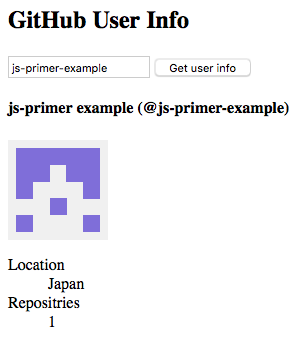
\includegraphics[width=100mm]{fig/fig-5.png}
\caption{完成したアプリケーション}
\end{figure}

\hypertarget{section-checklist}{%
\subsection{このセクションのチェックリスト}\label{section-checklist}}

\begin{itemize}
\item
  HTMLの組み立てと表示の処理を\texttt{createView}関数と\texttt{displayView}関数に分離した
\item
  \texttt{main}関数を宣言し、\texttt{fetchUserInfo}関数が返すPromiseのエラーハンドリングを行った
\item
  Promiseチェーンを使って\texttt{fetchUserInfo}関数をリファクタリングした
\item
  \href{../../../basic/async/README.md\#async-function}{Async Function}
  を使って\texttt{main}関数をリファクタリングした
\item
  \texttt{index.html}に\texttt{<input>}タグを追加し、\texttt{getUserId}関数でユーザーIDを取得した
\end{itemize}
